% Section content template for individual Educative lessons
% This file contains the actual content for a specific section
% Generated from Educative API section content

% Section: System Design Interview PDF
% Section ID: 6462532900225024
% Section Slug: system-design-interview-pdf
% Generated: 2025-12-08T15:45:00.738648

System Design has become a formal skillset focused on building and maintaining scalable, efficient distributed systems. Knowledge of System Design is now expected across a range of tech roles, from software engineers to technical project managers. To assess this skill, top tech companies, especially FAANG/MAANG, use the System Design Interview (SDI).
\\
Having conducted hundreds of System Design Interviews, the strategies below will help you prepare effectively. This lesson covers:

\begin{itemize}
\item
\protect\phantomsection\label{wKTN6XKe0u9XyD44o2wvW}
What makes System Design Interviews unique
\item
\protect\phantomsection\label{u5fR0aawZMJ5wLJvgxWaS}
An 8-week roadmap for SDI prep
\item
\protect\phantomsection\label{1iP4muntaoP34Pp-kAyZG}
How to prep effectively under time constraints
\end{itemize}
\\
Let\textquotesingle s get started.

\subsection{Understanding the System Design Interview}\label{IEEUYLuOq49AyLThJo2Yv}
\\
The System Design Interview isn't about writing lines of code but showing how an entire system would be built. It 's like being an architect sketching out the plans for a house.
\\
Open-ended problems are commonly given in the interview, such as "Design Quora" or "Design Uber." Companies ask these questions to evaluate the ability to navigate ambiguity and seek clarification.
\\
The first step is to evaluate existing knowledge based on the question, then ask clarifying questions about requirements and constraints. From there, it is possible to identify:

\begin{enumerate}
\item
\protect\phantomsection\label{uDpO8FKWP4cMIw8_yq6Zd}
What the system needs to do (i.e., functional requirements)
\item
\protect\phantomsection\label{fHAVGshcNp0CRx7WB8W6S}
How to make the system scale as it grows (i.e., non-functional requirements)
\end{enumerate}

\subsubsection{What makes System Design Interviews unique?}\label{uZn8NRVHaqkTVnUO1-VQA}

\begin{figure}[htbp]
 \centering
 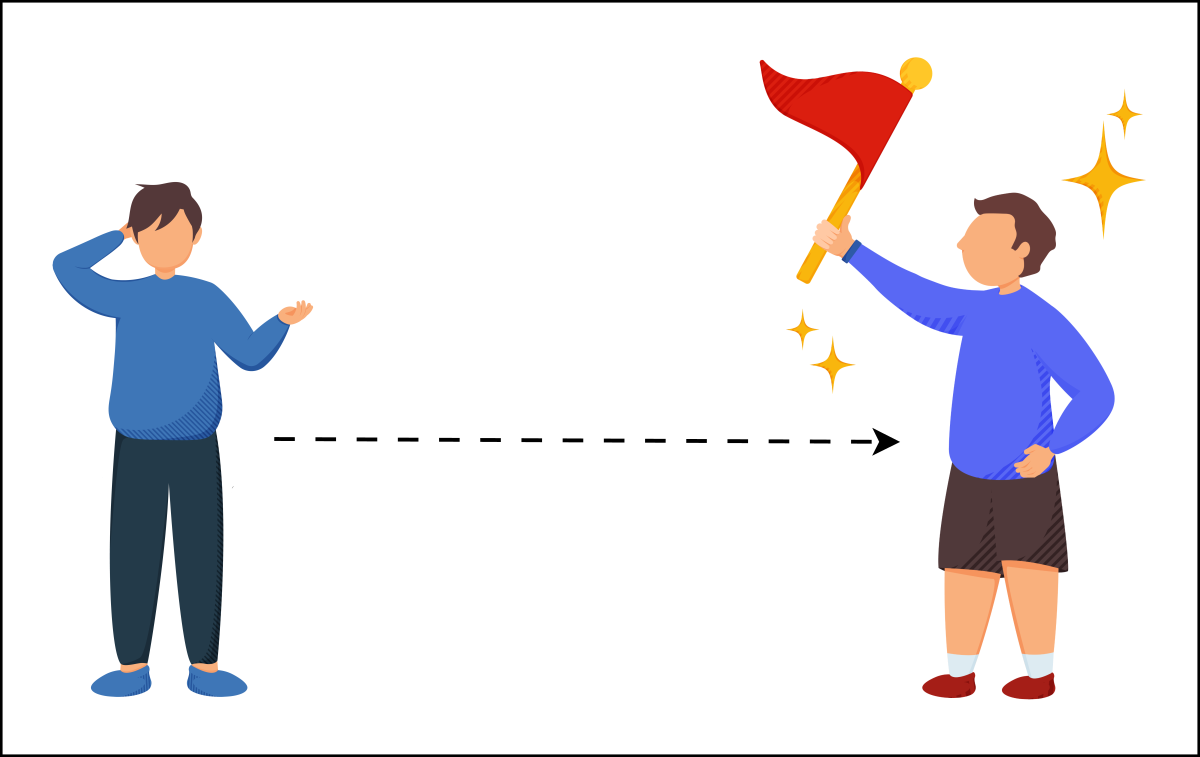
\includegraphics[width=0.15\textwidth]{Images/chapter_44/section_6462532900225024/4670706394988544.png}
 
\end{figure}

Unlike other technical interviews, the System Design Interview is heavily concerned with communication. There is no single right or wrong answer to a given System Design problem, and multiple paths can achieve the same goal.
\\
This means:

\begin{enumerate}
\item
\protect\phantomsection\label{ufspJnFwZ3tTuLFRQgJ8R}
The thought process is just as important as the final solution
\item
\protect\phantomsection\label{8Ot_pAouhEVQSbdD0szve}
Thinking must be communicated clearly throughout the interview
\end{enumerate}
\\
It is also recommended to limit the time spent designing during the interview to allow 5--10 minutes for discussion and feedback at the end. The communication-heavy nature of System Design Interviews allows candidates to showcase creativity, collaboration skills, and openness to feedback, highlighting both technical and soft skills.

\subsection{How to prepare for the System Design Interview}\label{Y86E8C9vRJ5pPm6-rKg7x}
\\
Preparing for the System Design Interview requires a strategic approach, balancing available time with the depth of preparation using targeted resources.
\\
Below is an 8-week roadmap to success as well as a strategy for streamlining prep.

\subsubsection{8-week System Design Interview roadmap}\label{VybsU8QFMUFeh3RhbAnYq}
\begin{quote}
\textbf{Note}: This roadmap can be adapted for any timeframe that suits the candidate.
\end{quote}
\\
\paragraph{Week 1: Laying the foundation}\label{MiFmt3qCz5W6-hzzFmLlX}
\\
If this is the first System Design Interview, start from scratch with a strong foundation for interview prep.
\\
Start with learning about:

\begin{itemize}
\item
\protect\phantomsection\label{czqVPfvooEx6ROhQtfNm-}
Operating systems, networking, and low-level design (OOD)
\item
\protect\phantomsection\label{ecELwgnS6DkLY97yRTUKx}
Key design principles and patterns
\item
\protect\phantomsection\label{Sekt1WrHLMjMpD4-R1-Kt}
Designing simple systems, such as a parking lot or a vending machine
\end{itemize}
\\
\paragraph{Week 2: Grokking distributed system concepts}\label{Jmxvn337WxBNpVPR21Ytm}

\begin{itemize}
\item
\protect\phantomsection\label{IkwRkJObFk1NuJrvzjMhd}
Understand microservices, the CAP theorem, consistency models, partitioning, sharding, replication, consensus, atomicity, and concurrency
\item
\protect\phantomsection\label{byfeloKr9jEHxvpBq8JyW}
Learn the key principles of System Design
\end{itemize}

\begin{center}
\fbox{\begin{minipage}{0.9\textwidth}
\centering
\vspace{0.2cm}
\textbf{\large Distributed system concepts and System Design fundamentals}
\\[0.2cm]
\textit{[Interactive Mind Map - See online version for interactive visualization]}
\vspace{0.2cm}
\end{minipage}}
\end{center}

\vspace{0.3cm}
\begin{itemize}
\item \textbf{System Design fundamentals}
\begin{itemize}
\item Microservices
\item Proxy servers
\item Caching
\item ACID transactions
\item Data partitioning
\item CAP \& PACELC theorem
\item Redundancy and replication
\item Storage and databases
\item System Design patterns
\item Load balancing
\item Availability
\item Scalability
\item Reliability
\item Fault tolerance
\item Consistency
\item Security
\item Low latency
\end{itemize}
\end{itemize}

\paragraph{Weeks 3-4: Learning building blocks}\label{7k8hp6Z24e35BpWOj0rro}
\\
System Design fundamentals are the building blocks of any successful system, shaping how a platform scales, adapts, and performs under pressure. From smart load balancing to choosing the right database (SQL vs. No SQL) to ensuring fault tolerance, these principles empower the creation of systems that aren't just functional but future-proof and resilient.
\\
Focus on:

\begin{itemize}
\item
\protect\phantomsection\label{tjmqWT6x_1tUIHWmpilbu}
Back-of-the-envelope estimation for various workloads
\item
\protect\phantomsection\label{fGHfrFQitXTpWFPXlqtBM}
Basic building blocks such as DNS, load balancers, databases, key-value stores, and CDNs
\item
\protect\phantomsection\label{trxOoMtlGsrAfStXsZKQr}
Essential components such as caches, queuing systems, pub/sub, distributed search, rate limiters, task schedulers, sequencers, blob stores, distributed monitoring, and logging
\end{itemize}
\\
\paragraph{Weeks 5-6: Practice designing real-world systems}\label{fddGpMTaZkOFs7sT7Bhth}
\\
This is when common System Design Interview problems are tackled.
\\
Focus on:

\begin{itemize}
\item
\protect\phantomsection\label{-WfhBr6hnH2wyvRfpGQgs}
Practice common System Design problems (based on real-world systems)
\item
\protect\phantomsection\label{H-kkHicGvtnbFsEUfD9fs}
Learn design problems by category to effectively tackle similar challenges
\end{itemize}
\\
Some of the most commonly asked System Design Interview questions at FAANG include:

\begin{table}[htbp]
\centering
\small
\adjustbox{max width=\textwidth}{
\begin{tabular}{|p{0.248\textwidth}|p{0.236\textwidth}|p{0.237\textwidth}|p{0.229\textwidth}|}
\hline
\href{https://www.educative.io/courses/grokking-the-system-design-interview/system-design-whatsapp}{Design a messenger app} & \href{https://www.educative.io/courses/grokking-the-principles-and-practices-of-advanced-system-design/introduction-to-gfs}{Design a distributed file system} & \href{https://www.educative.io/courses/grokking-the-api-design-interview/chess-api-design-ai-mentor-beta}{Design a chess game} & \href{https://www.educative.io/courses/grokking-the-system-design-interview/system-design-the-typeahead-suggestion-system}{Design a typeahead} \\
\hline
\href{https://www.educative.io/courses/grokking-the-system-design-interview/system-design-google-docs}{Design a collaborative editor} & \href{https://www.educative.io/courses/grokking-the-system-design-interview/system-design-the-distributed-search}{Design a search engine} \hfill\break & \href{https://www.educative.io/courses/grokking-the-system-design-interview/system-design-google-maps}{Design Google Maps} & \href{https://www.educative.io/courses/grokking-the-system-design-interview/system-design-instagram}{Design a newsfeed system} \\
\hline
\href{https://www.educative.io/courses/grokking-the-system-design-interview/system-design-instagram}{Design a social media app---Instagram/X} & \href{https://www.educative.io/courses/grokking-the-system-design-interview/system-design-the-content-delivery-network-cdn}{Design a content delivery network (CDN)} & \href{https://www.educative.io/courses/grokking-the-api-design-interview/requirements-of-the-gaming-api}{Design an online multiplayer game backend} & \href{https://www.educative.io/courses/grokking-the-system-design-interview/system-design-tinyurl}{Design a tinyURL service} \\
\hline
\href{https://www.educative.io/courses/grokking-modern-system-design-interview-for-engineers-managers/system-design-the-distributed-messaging-queue}{Design a distributed messaging queue} & \href{https://www.educative.io/courses/grokking-the-api-design-interview/requirements-of-the-stripe-api}{Design a payment gateway} & \href{https://www.educative.io/courses/grokking-the-api-design-interview/requirements-of-the-camelcamelcamel-api}{Design price tracking application--CamelCamelCamel} & \href{https://www.educative.io/courses/grokking-the-system-design-interview/system-design-web-crawler}{Design a web crawler} \\
\hline
\href{https://www.educative.io/courses/grokking-modern-system-design-interview-for-engineers-managers/system-design-tinyurl}{Design a URL-shortening service} & \href{https://www.educative.io/courses/grokking-the-system-design-interview/system-design-youtube}{Design a video streaming service} & \href{https://www.educative.io/courses/grokking-the-system-design-interview/system-design-the-distributed-cache}{Design a distributed cache system} & \href{https://www.educative.io/courses/grokking-the-system-design-interview/system-design-uber}{Design a ride-hailing service} \\
\hline
\href{https://www.educative.io/blog/system-design-interview-questions}{Design a food delivery system---Uber Eats} & \href{https://www.educative.io/blog/system-design-interview-questions}{Design a reservation system---OpenTable} & \href{https://www.educative.io/blog/system-design-interview-questions}{Design recommendation engine} & \href{https://www.educative.io/blog/system-design-interview-questions}{Design a comments moderation system} \\
\hline
\end{tabular}
}
\end{table}

\begin{quote}
\textbf{Note:} Some companies ask targeted questions according to the problems they currently face with their products, requiring research and understanding of the company\textquotesingle s products and design challenges.
\end{quote}
\\
\paragraph{Week 7: Revising and deep diving into design problems}\label{7ergIgM7jU-B_RYrb_zbW}
\\
There\textquotesingle s no right or wrong answer when it comes to System Design. This step is essential to learning how to navigate the nuances of designing scalable systems by building problem-solving skills and perspective.
\\
Focus on:

\begin{itemize}
\item
\protect\phantomsection\label{bK0njiedj34gZG9CJpfvT}
Understand trade-offs of different architectures and practice explaining designs clearly
\item
\protect\phantomsection\label{7Chr4preYZcuSnqIESPyA}
Revise complex scenarios and consider alternative optimal solutions
\end{itemize}
\\
\paragraph{Week 8: Practice with mock interviews}\label{oKVwCnIZ4xXocXOaZ8tHC}
\\
This interview assesses the ability to see the big picture and create a solid system ready for anything. This involves hashing out details like data storage, communication between app components, and handling high user loads.
\\
That said, all ourhard work is wasted if we can\textquotesingle t effectively communicate our thinking. To get used to discussing our thought process and ensure the interview goes smoothly, we need to focus on:

\begin{itemize}
\item
\protect\phantomsection\label{ZpU3tre4_IzU0XDtoJ4tT}
Taking mock interviews to simulate real-world scenarios
\item
\protect\phantomsection\label{xD0DVqFc26dxcKSLFE-E8}
Getting feedback and improving iteratively
\end{itemize}

\begin{center}\rule{0.5\linewidth}{0.5pt}\end{center}
\\
\emph{This free PDF goes deeper into this roadmap and resources to help you learn each concept. You can download it below.}

\begin{center}\rule{0.5\linewidth}{0.5pt}\end{center}

\subsubsection{Short on time? Practice problems by category}\label{WbaLnJWEWPAAk49aJmy8V}
\\
Practicing designing real-world systems is crucial to interview prep. That said, there is an endless pool of practice problems that we could do ---~and we don\textquotesingle t have an endless amount of time.
\\
A great way to streamline our prep is to practice problems by category, rather than trying to maximize individual problems.
\\
The thing is: many systems share similar goals. For instance, YouTube, Netflix, or Amazon Prime Video all belong to a broader category of video streaming services, which share similar requirements, including:

\begin{itemize}
\item
\protect\phantomsection\label{Ull3GwmJxqiR3li_OX_D2}
Allowing users to stream and search videos
\item
\protect\phantomsection\label{dc-iGnhIhP0GiCQoLWhx8}
High availability and reliability
\end{itemize}
\\
In a crunch, this means that designing YouTube prepares us to design other video streaming services like Netflix, etc.
\\
The main categories and design problems are listed below:

\begin{center}
\fbox{\begin{minipage}{0.9\textwidth}
\centering
\vspace{0.2cm}
\textbf{\large The five main categories of System Design problems}
\\[0.2cm]
\textit{[Interactive Mind Map - See online version for interactive visualization]}
\vspace{0.2cm}
\end{minipage}}
\end{center}

\vspace{0.3cm}
\begin{itemize}
\item \textbf{Video streaming systems}
\begin{itemize}
\item YouTube
\item Netflix
\item Amazon
\item Spotify
\item Twitch
\end{itemize}
\end{itemize}
\begin{itemize}
\item \textbf{Real-time communication systems}
\begin{itemize}
\item WhatsApp (Messaging)
\item Slack (Real-time communication)
\item Zoom (Video conferencing)
\item Discord (Voice, text, and video communication)
\item Online multiplayer gaming (Fortnite, Call of Duty)
\end{itemize}
\end{itemize}
\begin{itemize}
\item \textbf{Ride-hailing and location systems}
\begin{itemize}
\item Uber system
\item Lyft system
\item Google maps
\item Apple maps
\item DoorDash/Uber Eats
\end{itemize}
\end{itemize}
\begin{itemize}
\item \textbf{Feed-based social network systems}
\begin{itemize}
\item Instagram system
\item TikTok system
\item Facebook reels system
\item Twitter/X
\end{itemize}
\end{itemize}
\begin{itemize}
\item \textbf{File storage and sharing system}
\begin{itemize}
\item Dropbox (File sharing)
\item Google Drive (Cloud storage)
\item iCloud (Personal cloud storage)
\item OneDrive (File syncing and storage)
\item Dropbox system
\item Google Drive system
\end{itemize}
\end{itemize}

By practicing problems by categories, one canmaster key principles that apply across a handful of problems (and save time to prep for other key rounds in the interview process).

\subsubsection{}\label{B9iXWCFjL573rjdAF7HZt}

% End of section content